\documentclass{beamer}
\beamertemplatenavigationsymbolsempty
\usecolortheme{beaver}
\setbeamertemplate{blocks}[rounded=true, shadow=true]
\setbeamertemplate{footline}[page number]
%
\usepackage[utf8]{inputenc}
\usepackage[english,russian]{babel}
\usepackage{amssymb,amsfonts,amsmath,mathtext}
\usepackage{subfig}
\usepackage[all]{xy} % xy package for diagrams
\usepackage{array}
\usepackage{multicol}% many columns in slide
\usepackage{hyperref}% urls
\usepackage{hhline}%tables
% Your figures are here:
\graphicspath{ {../fig/} }

%----------------------------------------------------------------------------------------------------------
\title[\hbox to 56mm{Итеративное улучшение}]{Итеративное улучшение тематической \\ модели с обратной связью от пользователя}
\author[А.\,И. Горбулев]{Алексей Ильич Горбулев}
\institute{Московский физико-технический институт}
\date{\footnotesize
\par\smallskip\emph{Курс:} Моя первая научная статья/Группа Б05-021а
% Консультировался с В. А. Алексеевым по следующему поводу, так как схема такова: студент с Алексеевым, Алексеев с Воронцовым
\par\smallskip\emph{Эксперт:} д. ф.-м. н. К.\,В.~Воронцов
\par\smallskip\emph{Консультант:} В.\,А.~Алексеев
\par\bigskip\small 2023}
%----------------------------------------------------------------------------------------------------------
\begin{document}
%----------------------------------------------------------------------------------------------------------
\begin{frame}
\thispagestyle{empty}
\maketitle
\end{frame}
%-----------------------------------------------------------------------------------------------------
\begin{frame}{Доклад с одним слайдом}

\begin{columns}[c]
\column{0.6\textwidth}
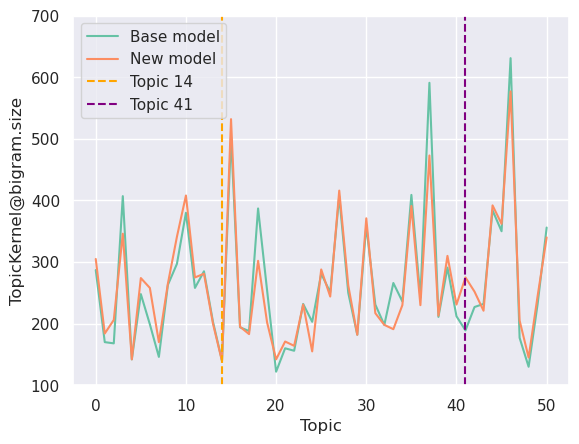
\includegraphics[width=1.0\textwidth]{figures/topickernel_bigram_size.png}
    
\column{0.4\textwidth}
    Используемые библиотеки:
    \begin{itemize}
        \item BigARTM
        \item TopicNet
    \end{itemize}
    {\footnotesize Цель улучшения модели: покрытие релевантными темами как можно большего числа документов}
\end{columns}

\bigskip
{\footnotesize Коллекция текстов основана на новостях с сайта Lenta.ru за период с $1999$ по $2019$ год. Для экспериментов используется часть из данного набора.}
\end{frame}


%----------------------------------------------------------------------------------------------------------
\end{document} 